\documentclass{beamer}

\usepackage[T2A]{fontenc}
\usepackage[utf8]{inputenc}
\usepackage[english,russian]{babel}
\usepackage{amssymb,amsfonts,amsmath,amsthm,mathtext}
\usepackage{cite,enumerate,float,indentfirst}

\usepackage{tikz-qtree,tikz-qtree-compat}        % regular trees (e.g. GB style)
\usepackage{tikz-dependency}   % dependency trees (bracket style)
\usepackage{gb4e}              % numbered lists for linguistic examples (IMPORTANT: If you use gb4e package, let it be the last \usepackage call in the document's preamble. Otherwise you may get exceeded parameter stack size error.)

\graphicspath{{images/}}

\usetheme{Rochester}
\usecolortheme{seagull}

\setbeamertemplate{footline}{\scriptsize{\hspace*{0.4cm}\insertframenumber}\vspace*{0.3cm}}
\beamertemplatenavigationsymbolsempty

\errorcontextlines 10000


\begin{document}

\title{\large{\sc Слабые контекстно-зависимые языки}}
\author{Константин Соколов}
%\institute[]{СПбГПУ}
%\date{Санкт-Петербург, 2015} 

\begin{frame}
    \thispagestyle{empty}
    \titlepage
\end{frame}


% 1. Трансформационная грамматика Хомского
\begin{frame}{}
\begin{center}
	\textbf{Трансформационная грамматика Н. Хомского}
\end{center}
\end{frame}

\begin{frame}{}
\begin{center}
	\begin{figure}[H]
		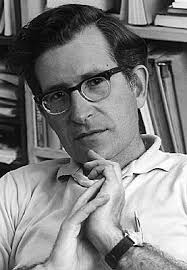
\includegraphics[scale=0.5]{chomsky.jpg} 
	\end{figure}
\end{center}
\smallskip
\begin{center}
Н.~Хомский. Синтаксические структуры, 1957
\end{center}
\end{frame}

\begin{frame}[fragile]{Грамматика составляющих -- I}
\begin{tiny}
\begin{center}
\Tree [.NP [.Adj золотые ] [.N пряди ] [.NP [.AP [.Adj склоняющейся ] [.PP [.Prep за ] [.NP [.Adj редкой ] [.N вещью ] ] ] ] [.N красавицы, ] [.AP [.Adj роющейся ] [.PP [.Prep меж ] [.NP [.N коробок ] ] ] ] ] ]
\end{center}
\end{tiny}
\end{frame}

\begin{frame}{Грамматика составляющих -- II}
\begin{small}
\begin{itemize}
    \item $S$ -- линейно упорядоченое множество слов
    \item размеченная система составляющих $C$ -- мн-во отрезков $S$, т.\,ч.
        \begin{itemize}
            \item $S \in C$
            \item если $A, B \in C$, то либо $A \subset B$, либо $B \subseteq A$, либо $A \cap B = \varnothing$
            \item $K$ -- множество категориальных символов
            \item каждому $c \in C$ приписан единственный $k \in K$
        \end{itemize}
    \item если $A \subset B$, то $B$ доминирует над $A$, $A$ -- составляющая $B$
\end{itemize}
\end{small}
\end{frame}

\begin{frame}{Грамматика составляющих -- III}
Структурные отношения:\\
\medskip
\begin{small}
\begin{itemize}
    \item если $A \subset B$, то $B$ доминирует над $A$, $A$ -- составляющая $B$
    \item если $A \subset B$ и не существует такого $C$, что $A \subset C \subset B$, \\то $A$ -- непосредственная составляющая $B$
\end{itemize}
\end{small}
\end{frame}

\begin{frame}{Трансформационная грамматика -- I}
\begin{quote}
Язык состоит из небольшого, возможно конечного, ядра основных предложений со структурой из непосредственных составляющих [\dots] и из множества трансформаций, которые можно применять к предложениям ядра или к предложениям, ранее полученным в результате трансформаций, для того чтобы производить новые и более сложные предложения из элементарных компонент.
\end{quote}
\begin{flushright}
Н. Хомский. Три модели описания языка. (1956)
\end{flushright}
\end{frame}

\begin{frame}{Трансформационная грамматика -- II}
\begin{scriptsize}
\begin{center}
\Tree [.VP [.Verb [.V turn ] [.Prt out ] ] [.NP [.Determ [.Quant some of ] [.Art the ] ] [.N lights ] ] ] \hspace{15pt}
\Tree [.VP [.Verb [.V turn ] ] [.NP [.Determ [.Quant some of ] [.Art the ] ] [.N lights ] ] [.Prt out ] ]
\end{center}
\end{scriptsize}
\end{frame}


%%%%%%%%%%%%%%%%%%%%%%%%%%%%%%%%
%   2. Недостаточность CFG
%%%%%%%%%%%%%%%%%%%%%%%%%%%%%%%%

\begin{frame}{}
\begin{center}
	\textbf{Недостаточность CFG}
\end{center}
\end{frame}

\begin{frame}{Недостаточность CFG}
\begin{itemize}
    \item Н.~Хомский. Синтаксические структуры, 1957
    \item G. Pullum, G. Gazdar. Natural languages and context-free languages, 1982
    \item Shieber M., Evidence against the context-freeness of natural language, 1987
\end{itemize}
\end{frame}

\begin{frame}{Перекрестные зависимости в голландском языке}
\begin{scriptsize}
\begin{exe}
	\ex 
		\gll $\ldots$ dat Jan Piet {de kinderen} zag helpen zwemmen\\
             $\ldots$ что Ян Пит дети видел помогать плавать\\
		\glt $\ldots$ \textit{что Ян видел, как Пит помогал детям плавать}
\end{exe}	
\end{scriptsize}

\begin{dependency}[theme = simple]
   \begin{deptext}[column sep=1em]
      $\ldots$ dat \& Jan \& Piet \& de kinderen \& zag \& helpen \& zwemmen \\
   \end{deptext}
   \depedge{1}{5}{}
   \depedge{5}{2}{}
   \depedge{5}{6}{}
   \depedge[edge start x offset=6.5pt]{6}{3}{}
   \depedge{6}{7}{}
   \depedge[edge start x offset=6.5pt]{7}{4}{}
\end{dependency}\\
\bigskip
\begin{center}
$L_1 = \{ww \, | \, w \in \{a, b, c\}^+\}$ (\textit{copy language}), $abcabc \in L_1$
\end{center}
\end{frame}

\begin{frame}{Перекрестные зависимости в швейцарском немецком}
\begin{scriptsize}
\begin{exe}
	\ex 
		\gll $\ldots$ das mer {em Hans}$_i$ {es huus}$_j$ h\"{a}lfed$_i$ aastriiche$_j$ \\
             $\ldots$ что мы Ганс-DAT дом-ACC помогали красить\\
		\glt $\ldots$ \textit{что мы помогали Гансу красить дом}
\end{exe}	
\end{scriptsize}

\begin{dependency}[theme = simple]
   \begin{deptext}[column sep=1em]
        $\ldots$ \& das \& mer \& em Hans \& es huus \& h\"{a}lfed \& aastriiche \\
   \end{deptext}
   \depedge{2}{6}{}
   \depedge{6}{3}{}
   \depedge[edge start x offset=-3pt]{6}{4}{}
   \depedge{6}{7}{}
   \depedge[edge start x offset=6.5pt]{7}{5}{}
\end{dependency}\\
\end{frame}

\begin{frame}{Скрэмблинг в немецком языке}
\begin{scriptsize}
\begin{exe}
	\ex 
		\gll dass {des Verbrechens}$_i$ {der Detektiv}$_j$ {den Verd\"{a}chtigen}$_i$ {dem Klienten}$_j$ {zu \"{u}berf\"{u}hren}$_i$ {versprochen hat}$_j$\\
             что преступление-GEN детектив-NOM подозреваемый-ACC клиент-DAT доказать пообещал\\
		\glt \textit{что детектив пообещал клиенту доказать вину подозреваемого}
\end{exe}	
\end{scriptsize}
\medskip
$L_2 = \{\pi(w')w \, | \, w = a_1 \dots a_n \in \{a, b, c\}^*\}, w' = a_1^{k_1} \ldots a_n^{k_n}$, где $k_i$ -- партиципант $a_j$, $\pi$ -- перестановка\\
\smallskip
$ababab, aabbab, abbaab, babaab, \ldots \in L_2$
\end{frame}

\begin{frame}{Согласование и гэппинг в английском}
\begin{scriptsize}
\begin{exe}
	\ex 
		\gll John likes $\varnothing_i$ and Tom hates broccoli$_i$ \\
             Джон любит {} и Том ненавидит брокколи\\
		\glt \textit{Джон любит, а Том ненавидит брокколи}
\end{exe}	
\begin{exe}
	\ex 
		\gll Mary always orders$_i$ wine, and Sally $\varnothing_i$ beer \\
             Мэри всегда заказывает вино, а Сэлли {} пиво \\
		\glt \textit{Мэри всегда заказывает вино, а Сэлли -- пиво}
\end{exe}
\begin{exe}
	\ex 
		\gll *Mary $\varnothing_i$ wine, and Sally always orders$_i$ beer \\
             Мэри {} вино, а Сэлли всегда заказывает пиво \\
		\glt \textit{Мэри всегда заказывает вино, а Сэлли -- пиво}
\end{exe}
\end{scriptsize}
\end{frame}


%%%%%%%%

\begin{frame}{Shieber (1987) -- I}
Пусть $L$ -- множество предложений швейцарского немецкого. Рассмотрим следующее предложение:\\ 
\begin{scriptsize}
\begin{exe}
	\ex 
		\gll Jan s\"{a}it das mer d'chind {em Hans} {es huus} {haend wele} laa h\"{a}lfe aastriiche \\
             Ян говорит что мы дети-ACC Ганс-DAT дом-ACC хотели позволить помогать красить \\
		\glt \textit{Ян говорит, что мы хотели позволить детям помочь Гансу красить дом}
\end{exe}
\end{scriptsize}
\bigskip

Построим гомоморфизм $f : L \to \{a, b, c, d, w, x, y, z\}^*$\\
\begin{center}
\begin{footnotesize}
\texttt{$\textnormal{``d'chind''} \mapsto a, \textnormal{``em Hans''} \mapsto b, \textnormal{``laa''} \mapsto c$\\
$\textnormal{``h\"{a}lfe''} \mapsto d, \textnormal{``Jan s\"{a}it das mer''} \mapsto w$\\
$\textnormal{``es huus haend wele''} \mapsto x, \textnormal{``aastriche''} \mapsto y$\\
$f(\_) = z$ в остальных случаях}
\end{footnotesize}
\end{center}
\end{frame}

\begin{frame}{Shieber (1987) -- II}
Гомоморфный образ КС-языка -- КС-язык. {\small \textit{(теорема №1)}}\\
\bigskip
Если $L$ -- КС-язык, то $f(L)$ -- тоже КС-язык. {\small \textit{(по теореме №1)}}\\
\bigskip
Строим пересечение $L_{SD} = f(L) \cap \{ wa^*b^*xc^*d^*y \} =$\\ $= \{ wa^ib^jxc^id^jy \, | \, i, j \geq 0 \}$.\\
\bigskip
Пересечение контекстно-свободного языка с регулярным языком -- контекстно-свободный язык. {\small \textit{(теорема №2)}}\\
\bigskip
Но $L_{SD} \cap \{ a^*b^*c^*d^* \} = \{ a^ib^jc^id^j \, | \, i, j \geq 0 \}$ -- не КС-язык.\\ {\small \textit{(по лемме о разрастании)}}\\
\bigskip
Противоречие, поэтому $L$ -- не КС-язык.
\end{frame}


% 3. Джоши, mild context sensitivity
\begin{frame}{}
\begin{center}
	\textbf{Mild Context Sensitivity}
\end{center}
\end{frame}

\begin{frame}{Joshi (1985) -- I}
\begin{center}
	\begin{figure}[H]
		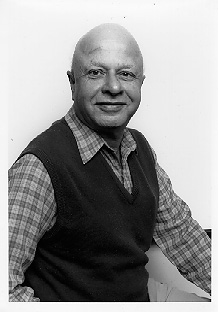
\includegraphics[scale=0.5]{joshi.jpg} 
	\end{figure}
\end{center}
\smallskip
\begin{center}
{\small Joshi, A. (1985) Tree adjoining grammars: How much context-sensitivity is required to provide reasonable structural descriptions?}
\end{center}
\end{frame}

\begin{frame}{Joshi (1985) -- II}
Класс $\mathcal{L}$ языков \textit{слабо контекстно-зависим} если и только если\\
\smallskip
\begin{itemize}
    \item $\mathcal{L}$ содержит все контекстно-свободные языки
    \item $\mathcal{L}$ может описывать перекрестные зависимости (существует $n \geq 2$ т.\,ч. $\{ w^k \, | \, w \in T^* \} \in \mathcal{L}$ для всех $k \leq n$)
    \item языки в классе $\mathcal{L}$ должны парситься за полиномиальное время
    \item языки в классе $\mathcal{L}$ обладают свойством ``константного роста'' (в упорядоченном по длине списке слов в языке $L \in \mathcal{L}$ длина слов растет линейно)
\end{itemize}
\end{frame}

% 4. Нетрансформационные формализмы в классе MCSG
%       TAG; extended domain of locality
%       CCG; AB, CCG, MMCCG
\begin{frame}{}
\begin{center}
	\textbf{Нетрансформационные формализмы в классе MCSG}
\end{center}
\end{frame}

\begin{frame}{Tree Adjoining Grammar -- I}
Грамматика присоединения деревьев (TAG) задается как\\
\medskip
\begin{itemize}
    \item множество элементарных деревьев
        \begin{itemize}
            \item начальные деревья        
            \item вспомогательные деревья (содержат ровно один отмеченный лист, т.н. \textit{foot node})
        \end{itemize}
    \item две операции
        \begin{itemize}
            \item подстановка (\textit{substitution}) -- замена листа в одном дереве другим деревом
            \item присоединение (\textit{adjunction}) -- перевешивание поддерева на отмеченный лист во вспомогательном дереве
        \end{itemize}
    \item пометки на узлах в дереве для контроля композиции
        \begin{itemize}
            \item присоединение запрещено (\textit{null adjunction, NA})
            \item присоединение только деревьев из конкретного набора
        \end{itemize}
\end{itemize}
\end{frame}

\begin{frame}{Tree Adjoining Grammar -- II}
Присоединение вспомогательного дерева\\
\bigskip
\begin{center}
\begin{scriptsize}
\Tree [.S [.NP John ] [.VP [.V laughs ] ] ] \hspace{15pt}
\Tree [.VP [.Adv always ] [.VP^* ] ] \hspace{15pt}
$\Rightarrow$ \hspace{15pt}
\Tree [.S [.NP John ] [.VP [.Adv always ] [.VP [.V laughs ] ] ] ]
\end{scriptsize}
\end{center}
\end{frame}

\begin{frame}{Tree Adjoining Grammar -- III}
TAG для $\{ ww \, | \, w \in \Sigma^* \}$\\
\bigskip
\begin{center}
\begin{scriptsize}
$\alpha$) \Tree [.S $\epsilon$ ] \hspace{15pt}
$\beta_a$) \Tree [.S_{NA} a [.S S_{NA}^* a ] ] \hspace{15pt}
$\beta_b$) \Tree [.S_{NA} b [.S S_{NA}^* b ] ]
\end{scriptsize}
\end{center}
\end{frame}

\begin{frame}{Tree Adjoining Grammar -- IV}
TAG для перекрестных зависимостей\\
\smallskip
\begin{center}
\begin{tikzpicture}
\tikzset{level distance=20pt, sibling distance=5pt}
\begin{tiny}
\Tree [.S_{NA} [.S_{OA} \qroof{de kinderen}.NP 
                        [.VP [.V_i $\epsilon$ ] ] ] 
               [.V_i zwemmen ] ] 
\end{tiny}
\end{tikzpicture}        
\begin{tikzpicture}
\tikzset{level distance=20pt, sibling distance=5pt}
\begin{tiny}
\Tree [.S_{NA} [.S_{OA} [.NP Marie ]
                        [.VP S_{NA}^* [.V_i $\epsilon$ ] ] ] 
               [.V_i leren ] ] \hspace{1pt}  
\end{tiny} 
\end{tikzpicture}             
\begin{tikzpicture}
\tikzset{level distance=20pt, sibling distance=5pt}
\begin{tiny}
\Tree [.S_{NA} [.S_{OA} [.NP Piet ]
                        [.VP S_{NA}^* [.V_i $\epsilon$ ] ] ] 
               [.V_i helpen ] ] \hspace{1pt} 
\end{tiny}  
\end{tikzpicture}          
\begin{tikzpicture}
\tikzset{level distance=20pt, sibling distance=5pt}
\begin{tiny}
\Tree [.S_{NA} [.NP Jan ]
               [.VP S_{NA}^* [.V sag ] ] ] 
\end{tiny}
\end{tikzpicture}               
\end{center}
\end{frame}

\begin{frame}{Комбинаторные категориальные грамматики -- I}
Простейший вариант КГ (т.н. AB-исчисление) задается как\\
\medskip
\begin{itemize}
    \item синтаксические категории (словарь):
      \begin{itemize}
        \item атомарные категории: $s$, $np$, \ldots
        \item составные категории: $s/np$, $s \backslash np$, $np/np$, $(s/np) \backslash (s/np)$, \ldots
        \item две операции для построения составных категорий
          \begin{itemize}
            \item $\backslash$ --- <<аргумент слева>>
            \item $/$ --- <<аргумент справа>>
          \end{itemize}
        \item пример: $love \vdash (s \backslash np) / np, love \vdash np$
      \end{itemize}
      \medskip
    \item сочетаемостные правила:
      \begin{eqnarray*}
        (X / Y)~Y &\rightarrow_{>}& X \\
        Y~(X \backslash Y) &\rightarrow_{<}& X
      \end{eqnarray*}
\end{itemize}
\end{frame}

\begin{frame}{Комбинаторные категориальные грамматики -- II}
\begin{center}
	\begin{figure}[H]
		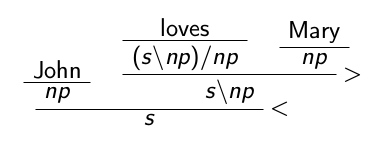
\includegraphics[scale=0.5]{ccg1.png} 
	\end{figure}
\end{center}
\end{frame}

\begin{frame}{Комбинаторные категориальные грамматики -- III}
  
  \begin{itemize}
    \item $\lambda$-термы можно строить из других $\lambda$-термов с помощью
        \textit{комбинаторов} (функций без свободных переменных)
  \end{itemize}
  
  Идея:\\
  \medskip
  \begin{itemize}
    \item выберем подходящий набор комбинаторов, которые позволяют 
          из одних термов строить другие
    \item типу аргумента (исходного терма) сопоставляется новый тип,
          тип значения
    \item добавим к AB-исчислению правила, которые будут по тем же
          законам преобразовывать синтаксические категории
  \end{itemize}
\end{frame}  

\begin{frame}{Комбинаторные категориальные грамматики -- IV}
Комбинаторная логика:\\
\medskip
  \begin{itemize}
    \item подъем типа (type-raising):\\
         $T~x \equiv \lambda f.f~x$
    \item композиция функций (function composition):\\
         $B~f~g \equiv \lambda x.f~(g~x)$
    \item подстановка (substitution):\\
         $S~f~g \equiv \lambda x.f~x~(g~x)$
  \end{itemize}
\end{frame}

\begin{frame}{Комбинаторные категориальные грамматики -- V}
Подъем типа:
\begin{eqnarray*}
X &\rightarrow_{>_T}& Y / (Y \backslash X) \\
X &\rightarrow_{<_T}& Y \backslash (Y / X) 
\end{eqnarray*}
  
Композиция:
\begin{eqnarray*}
(X / Y) ~~(Y / Z)  &\rightarrow_{>_B}& X/Z  \\
(Y / Z) ~~(X \backslash Y)  &\rightarrow_{<_B}& X \backslash Z
\end{eqnarray*}  
  
Подстановка:
  \begin{eqnarray*}
  (Y / Z)~~(X \backslash Y) / Z) &\rightarrow_{<_{S_{\times}}}& X/Z 
  \end{eqnarray*}  
\end{frame}

\begin{frame}{Комбинаторные категориальные грамматики -- VI}
\begin{center}
	\begin{figure}[H]
		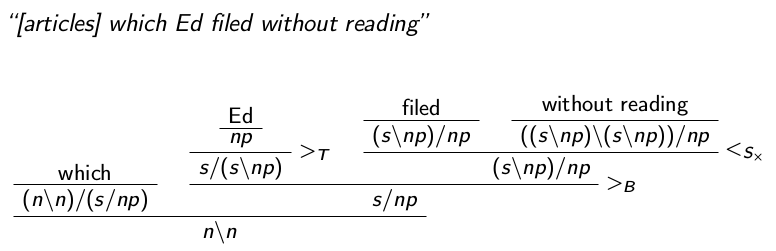
\includegraphics[scale=0.4]{ccg2.png} 
	\end{figure}
\end{center}
\end{frame}

\begin{frame}{}
\begin{center}
	\textbf{Заключение}
\end{center}
\end{frame}

\begin{frame}{Beyond CFG}
Что известно о \textit{mildly context sensitive} языках\\
\bigskip 
\begin{itemize}
    \item TAG и CCG
        \begin{itemize}
            \item слабо эквивалентны друг другу (задают один и тот же класс языков, но структурные описания не совпадают)
            \item самые слабые формализмы в классе MCS
            \item парсятся за $O(n^6)$
        \end{itemize}
    \item самый выразительный формализм в классе MCS неизвестен
\end{itemize}
\end{frame}

\begin{frame}{}
    \thispagestyle{empty}
    \begin{center}
        {\large Спасибо!}
    \end{center}
\end{frame}


\end{document}
